\documentclass[letter]{article}
\usepackage{amsmath}
\usepackage{amssymb}
\usepackage{graphicx}

\setlength\oddsidemargin{0.25in}
\setlength\evensidemargin{0.25in}
\setlength\topmargin{0.0in}
\setlength\textheight{8in}
\setlength\textwidth{6in}
\setlength\parindent{0in}

\usepackage{fancyhdr}
\pagestyle{fancy}

\fancyhead[L]{Symmetries of the triangle}
\fancyhead[C]{Tech 411.05 {\em Patterns and Symmetry}}
\fancyhead[R]{\thepage}
\fancyfoot{}

\newcommand{\bx}{{\bf x}}
\newcommand{\Sa}{S_{\alpha}}
\newcommand{\Sb}{S_{\beta}}
\newcommand{\Sg}{S_{\gamma}}
\newcommand{\Sx}{S_x}
\newcommand{\Sy}{S_y}

\begin{document}

\section{Symmetries: the mathematics of patterns}

We all recognize the left-right symmetry of a face, or the black/white symmetry of a chessboard.
But as we've seen with the Escher patterns, there are more complicated kinds of symmetries.
To understand these more complicated symmetries, we need to describe them mathematically. 

\vspace{2mm}
{\bf Definition:} A shape is {\em symmetric} if it does not change under
a given a coordinate transformation. Such a coordinate transformation is called a
{\em symmetry} of the shape. The shape is {\em invariant} under the symmetry.

\vspace{2mm}
{\bf Example: a reflection symmetry}. The equilateral triangle below is invariant under
reflection about the vertical axis. Some points swap positions, such as $\alpha$ and $\gamma$.
But the shaded regions in the two plots contain the same points. 
\begin{center}
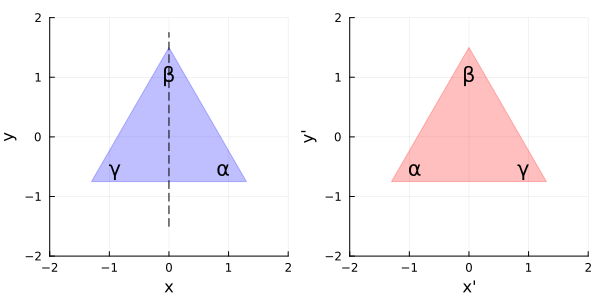
\includegraphics[width=0.7\textwidth]{triangle-sx-symmetry.png}
\end{center}
As we've seen in previous sessions, the coordinate transformation that performs this reflection
is $\bx' = \Sy \bx$ where $\bx = \begin{bmatrix} x \\ y \end{bmatrix}$ and
$\Sy = \begin{bmatrix} -1 & 0 \\ 0 & 1 \end{bmatrix}$. So $\Sy$ is a symmetry of the triangle.
Equivalently, the triangle is $\Sy$-symmetric.

\vspace{6mm}
In contrast the triangle is not invariant under reflection about the horizontal axis. The shaded 
regions in the two plots differ. The coordinate transformation for reflection about the horizontal
axis $\Sx = \begin{bmatrix} 1 & 0 \\ 0 & -1 \end{bmatrix}$. So $\Sx$ is not a symmetry
of the triangle, and the triangle is not $\Sx$-symmetric.
\begin{center}
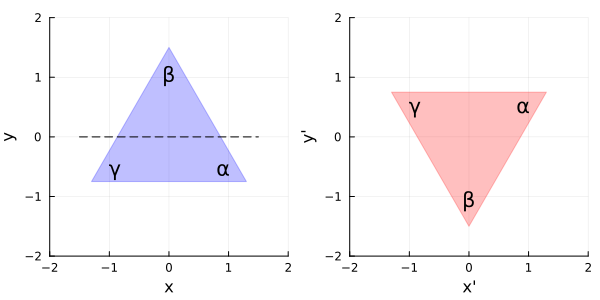
\includegraphics[width=0.7\textwidth]{triangle-sy.png}
\end{center}

\vspace{6mm}
{\bf Example: a rotation symmetry}
The triangle is invariant under the rotation $R_{2\pi/3}$, where
$R_{\theta} = \begin{bmatrix} \cos(\theta) & -\sin(\theta) \\ \sin(\theta) & \cos(\theta) \end{bmatrix}$
and thus 
$R_{2\pi/3} = \begin{bmatrix} \cos(2\pi/3) & -\sin(2\pi/3) \\ \sin(2\pi/3) & \cos(2\pi/3) \end{bmatrix}
= \begin{bmatrix} -1/2 & -\sqrt{3}/2 \\ \sqrt{3}/2 & -1/2 \end{bmatrix}$.
\begin{center}
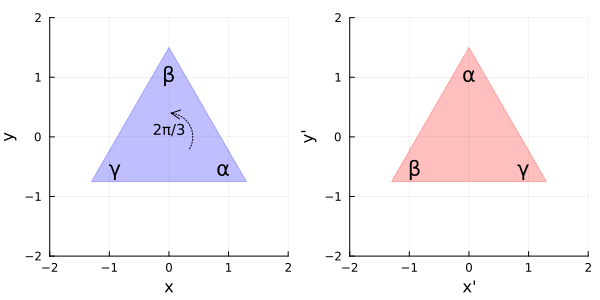
\includegraphics[width=0.7\textwidth]{triangle-R.png}
\end{center}
The triangle is thus $R_{2\pi/3}$-symmetric.

\vspace{2mm}
What other symmetries does the triangle have? We could also reflect it about the axis going
through any of the triangle's vertices (shown below), or rotate it any multiple of $2\pi/3$. 
\begin{center}
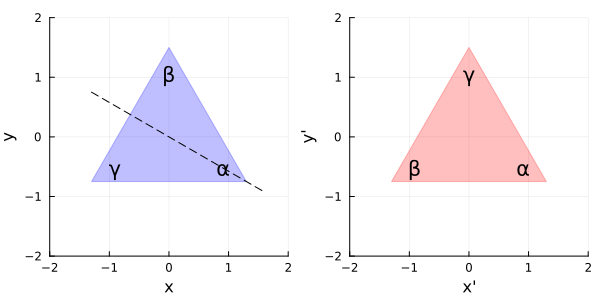
\includegraphics[width=0.7\textwidth]{triangle-Salpha.png}
\end{center}

\vspace{8mm}
\rule{\textwidth}{0.5pt}
{\bf Problem 1:} What are all the symmetries of the triangle?

\vspace{2mm} Use a cut-out, labeled triangle to figure out all possible rotations and reflections
that leave the triangle as a whole unchanged. For each, draw a picture of two triangles with
labeled vertices, like the ones above.

\vspace{2mm} You don't have to figure out the matrices that represent the symmetries. Just give
the symmetries names, like $\Sa$ for reflection about the axis going through vertex $\alpha$, and
$R_{2\pi/3}$ for rotation by $2\pi/3$. 

\vspace{2mm} Hint: the triangle has six symmetries. Don't forget the identity symmetry,
$I = R_0 = \begin{bmatrix} 1 & 0 \\ 0 & 1 \end{bmatrix}$.

\pagebreak
\vspace{2mm} {\bf Answers:}

\pagebreak

\section{Finding symmetries by substitution}

How can we know how many symmetries an object has, and how can we find all of them? 
There is a systematic way to answer these questions. Let $T$ be the set of all points
in the triangle,
\begin{align*}
T = \{\bx_1, \bx_2, \ldots\} = \left\{\begin{bmatrix} x_1 \\ y_1 \end{bmatrix}, \begin{bmatrix} x_2 \\ y_2 \end{bmatrix}, \ldots \right\}.
\end{align*}
Next let $ST$ represent the coordinate transformation $S$ applied to all the points in $T$,
\begin{align*}
  S\,T = S \, \{\bx_1, \bx_2, \ldots\} =  \{S\bx_1, S\bx_2, \ldots\}.
\end{align*}
If the triangle is unchanged by a coordinate transformation $S$, we have $T = S\, T$. For example,
the triangle's symmetry about the $y$ axis and its symmetry under rotation by $2\pi/3$ can be expressed
as
\begin{align*}
  T = \Sy\, T \quad \quad \text{and} \quad  \quad T = R_{2\pi/3}\, T.
\end{align*}
In words, the triangle is invariant under both $\Sy$ and $ R_{2\pi/3}$, and it
has these both as symmetries. 

\vspace{4mm}
Now here's the key idea:
{\bf We can find {\em all} the symmetries of the triangle by substitution!}

\vspace{4mm}
{\bf Example:} Since $T = R_{2\pi/3}\, T$ we can substitute $R_{2\pi/3}\, T$ for $T$ on the
right-hand side of the equation to get
\begin{align*}
  T &=  R_{2\pi/3}\, (R_{2\pi/3}\, T), \\
    & = (R_{2\pi/3} R_{2\pi/3})\, T, \\
    & = R_{2\pi/3}^2 \, T.
\end{align*}
Thus the triangle is invariant under two rotations by $2\pi/3$, or equivalently, one rotation by $4\pi/3$,
and is $R_{2\pi/3}^2 = R_{4\pi/3}$ symmetric.
\begin{center}
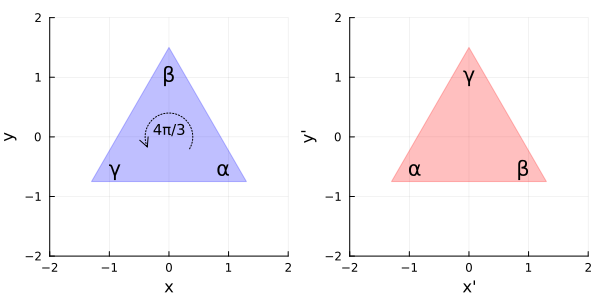
\includegraphics[width=0.7\textwidth]{triangle-R2.png}
\end{center}
$R_{4\pi/3}$ should be one of your answers for problem 1.


\pagebreak
From here on let's drop the subscripts, let $R = R_{2\pi/3}$ and $R^2 = R_{4\pi/3}$, so that our 
equations of the triangle's invariance under reflection and rotation are
\begin{align*}
  T = \Sy\, T \quad \quad \text{and} \quad  \quad T = R\, T,
\end{align*}
and the manipulations of the example above amount to $T = R\, T = R (R\, T) = R^2 T$. 


\vspace{4mm}
\rule{\textwidth}{0.5pt}
{\bf Problem 2:} Substituting $T = \Sy\,T$ into $T = R\,T$ gives $T = R (\Sy\, T)$. Since
matrix multiplication is associative, $T = (R \Sy) \,T$. The triangle thus has $R \Sy$
symmetry: it is invariant under reflection about the $y$ axis followed by rotation by $2\pi/3$.

\vspace{2mm}
Verify that your cut-out triangle is $R \Sy$-symmetric by performing the reflection
about the $y$ axis followed by the rotation, and seeing that the whole shape is unchanged.
Draw a picture that shows the transformation and symmetry. Of the symmetries you listed
for problem 1, which symmetry is the same as $R \Sy$?

\vspace{2mm}
{\bf Answer:}

\vspace{64mm}
\rule{\textwidth}{0.5pt}
{\bf Problem 3:}
Substituting $T = R\,T$ into $T = \Sy\,T$ gives $T = \Sy (R \,T) = (\Sy R) \,T$.
Thus the triangle is $\Sy R$ symmetric.

\vspace{2mm}
Verify that your cut-out triangle is $\Sy R$-symmetric by performing the rotation followed
by reflection about the $y$ axis. Draw a picture that shows the transformation and the
symmetry. Of the symmetries you listed for problem 1, which is the same as $\Sy R$?

\vspace{2mm}
{\bf Answer:}

\pagebreak
It is not hard to derive the equations
\begin{align*}
  T = R^m\, T, \quad \quad T = \Sy^n\, T, \quad \quad  T = R^m \Sy^n \, T,  \quad \quad T = \Sy^n R^m \, T
\end{align*}  
for any integers $m,n \geq 0$ from $T=T$ and repeated substitutions of $T = R\,T$ and $T = \Sy\,T$.

\vspace{2mm}
Note that since a repeated reflection undoes itself, $S_y^2 = I$. Thus there is no point of going
beyond $n=1$ in $\Sy^n$. Similarly, there is no point going beyond $m=2$ in $R^m$, since 
since three rotations by $2\pi/3$ is the same as rotation by zero. We will show in problem 5
that symmetries of the form $\Sy^n R^m$ are redundant with those of form $R^m \Sy^n$.

\vspace{4mm}
{\bf The complete set of symmetries of the triangle is thus $I, R, R^2, \Sy, R\Sy,$ and $R^2\Sy$.}

\vspace{4mm}
\rule{\textwidth}{0.5pt}
{\bf Problem 4:} For each of $I, R, R^2, \Sy, R\Sy,$ and $R^2\Sy$, perform the transformation on
the cut-out triangle, draw pictures, and indicate which of your answers from problem 1 is the same. 


\pagebreak

\section{Symmetry groups}

Just as rotation $R$ and reflection $\Sy$ can be performed in sequence to form the product $R \Sy$,
each of the symmetries of problem 4 can be performed in sequence to form a product.

\vspace{2mm}
\rule{\textwidth}{0.5pt}
{\bf Problem 5:} Using your cut-out triangle, fill out the multiplication table. Start with the triangle
in its original position, perform the transformation in the column, and then the transformation
in the row. Then look in your answers to problem 4, and see which of $I, R, R^2, \Sy, R\Sy,$ or
$R^2\Sy$ you got, and write that in the corresponding spot in the table.

\vspace{2mm}
For example, for transformation $\Sy$ (column) followed by transformation $R$ (row), you should
get $R \Sy$ as shown. 




\vspace{130mm}
This is the {\em group multiplication} table of the symmetries of the triangle. Note that
\begin{enumerate}
\item The product of any two symmetries is a symmetry. The set is closed under multiplication.
  \vspace{-2mm}
\item One of the symmetries is the identity $I$. 
  \vspace{-2mm}
\item The identity $I$ appears once in every row and every column: every symmetry has an inverse.
\end{enumerate}  
These, plus associativity of multiplication, are the key properties of a group.

\end{document}









1




























\begin{align}
  x' &= ax + by \\
  y' &= cx + dy \nonumber
\end{align}
where $a,b,c,$ and $d$ are constants determined by the rotation angle. 

\vspace{2mm}
{\bf Problem 1:} Figure out the values of $a,b,c,$ and $d$ as functions
of the rotation angle $\theta$. 

\vspace{2mm}
{\bf Strategy:} There are four unknowns $a,b,c,d$, so we need four equations to solve for them.
Choose a point on the original square, say vertex $\alpha$ at $(x,y) = (1,1)$. Use trigonometry
to find the position $(x',y')$ of vertex $\alpha$ after rotation as a function of the rotation angle
$\theta$. Then plug those values of $(x,y)$ and $(x',y')$ into the above equations. That gives
you two equations. Do the same for another point, say vertex $\beta$, to get two more equations.
Solve the four equations to get $a,b,c,d$ as trigonometric functions of $\theta$.

\newpage

\vspace{2mm}
{\bf Hint:} If you use the points $(x,y) = (0,1)$ and $(x,y) = (1,0)$ instead of the
vertices $\alpha$ and $\beta$, the trigonometry and algebra are much simpler.

\begin{center}
  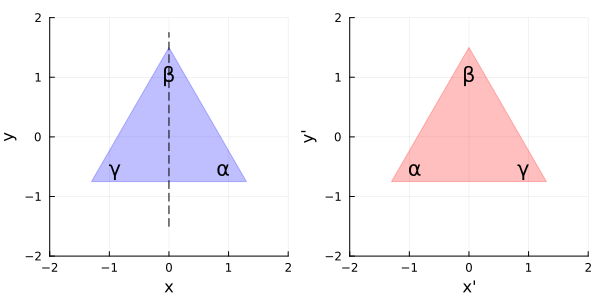
\includegraphics[width=0.75\textwidth]{triangle-sx-symmetry.png}
\end{center}

\newpage

{\bf Problem 2:} Rewrite your answer to problem 1 as a matrix-vector multiplication.

\vspace{2mm}
{\bf Guidance:} The equations 
\begin{align}
  x' &= ax + by \nonumber \\      
  y' &= cx + dy         \label{linreln_algebra}
\end{align}
can be written as a matrix-vector multiplication 
\begin{align}
  \begin{bmatrix} x' \\ y' \end{bmatrix}
  =
  \begin{bmatrix} a & b \\ c & d \end{bmatrix}                       
  \begin{bmatrix} x \\ y \end{bmatrix}.  \label{linreln_matrix}
\end{align}
This is just a graphical way to represent the original equations.

\vspace{3mm}
$\begin{bmatrix} x' \\ y' \end{bmatrix}$ and $\begin{bmatrix} x \\ y \end{bmatrix}$
are {\em vectors} representing the coordinates $(x',y')$ and $(x,y)$ as points on a plane.

\vspace{3mm}
$\begin{bmatrix} a & b \\ c & d \end{bmatrix}$ is a {\em matrix} that specifies
the functional relationship between the vectors $(x',y')$ and $(x,y)$.

\vspace{3mm}
Matrix-vector multiplication is defined by the ``across and down'' rule. For example,
the product 
\begin{align*}
  \begin{bmatrix} 2 & 1 \\ 3 & -4 \end{bmatrix}                       
  \begin{bmatrix} 5 \\ 6 \end{bmatrix} 
\end{align*}
is found by multiplying each entry {\em across} the first row of the matrix by the entries
going {\em down} the vector and adding,
\begin{align*}
  \begin{bmatrix} 2 & 1 \\  & \end{bmatrix}
  \begin{bmatrix} 5 \\ 6 \end{bmatrix}  \quad
  =
  \begin{bmatrix} 2 \cdot 5 + 1 \cdot 6 \\ \phantom{5} \end{bmatrix} 
  = 
  \begin{bmatrix} 16 \\  \phantom{5} \end{bmatrix},
\end{align*}
and then doing the same going across the bottom row of the matrix to get
\begin{align*}
  \begin{bmatrix}  \\  3 & -4 \end{bmatrix}
  \begin{bmatrix} 5 \\ 6 \end{bmatrix} \quad
  =
  \begin{bmatrix} \phantom{5} \\ 3 \cdot 5 - 4 \cdot 6 \end{bmatrix} 
  = 
  \begin{bmatrix} \phantom{16} \\  -9 \end{bmatrix}.
\end{align*}
Thus
\begin{align*}
  \begin{bmatrix} 2 & 1 \\ 3 & -4 \end{bmatrix}                       
  \begin{bmatrix} 5 \\ 6 \end{bmatrix}
  =
  \begin{bmatrix} 16 \\ -9\end{bmatrix}.                       
\end{align*}

Similarly, 
\begin{align}
  \begin{bmatrix} x' \\ y' \end{bmatrix}
  =
  \begin{bmatrix} a & b \\ c & d \end{bmatrix}                       
  \begin{bmatrix} x \\ y \end{bmatrix}
  =
  \begin{bmatrix} ax + by \\ cx + dy \end{bmatrix}.
\end{align}
This is just equation \ref{linreln_algebra} written as an equality of two vectors.
So to get your answer for problem 2, just substitute the trigonometric functions
for $a,b,c,d$ that you derived in problem 1 into equation \ref{linreln_matrix}.



\section{Reflections}

{\bf Problem 3:} Using similar methods as in problems 1 and 2, derive a matrix-vector
representation of reflection about the vertical axis. 

\begin{center}
%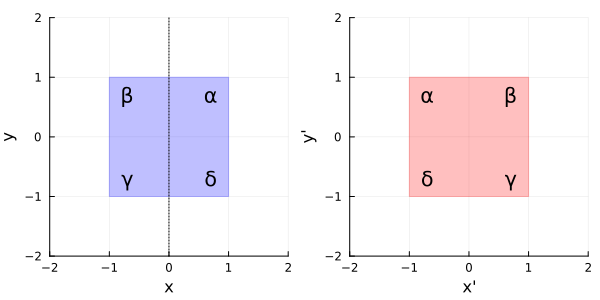
\includegraphics[width=0.75\textwidth]{xreflection.png}
\end{center}

Your answer will be of the form $
  \begin{bmatrix} x' \\ y' \end{bmatrix}
  =
  \begin{bmatrix} a & b \\ c & d \end{bmatrix}                       
  \begin{bmatrix} x \\ y \end{bmatrix}
$
with specific numeric values for $a,b,c,d$.

\newpage

{\bf Problem 4:} Do the same as problem 3 for reflection about the horizontal axis. 

\begin{center}
%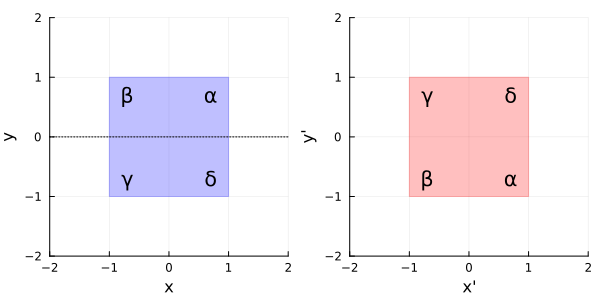
\includegraphics[width=0.75\textwidth]{yreflection.png}
\end{center}

\newpage

{\bf Problem 5 (challenge):} Derive a matrix-vector representation of a reflection
about a diagonal line at angle $\pi/4$ ($45^\circ$). 

\begin{center}
%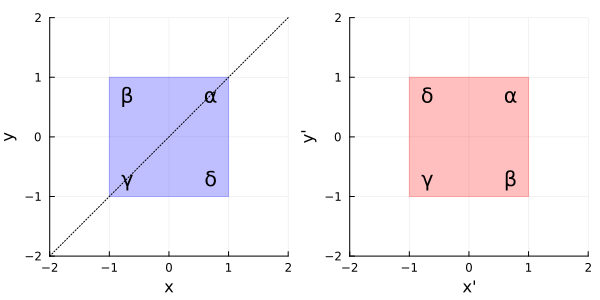
\includegraphics[width=0.75\textwidth]{diagonalreflection.png}
\end{center}
\newpage

\section{Chained transformations, matrix-matrix multiplication.}


Here we see a rotation of a square by $\theta = \pi/6$ followed by a reflection
about the vertical axis.

\begin{center}
%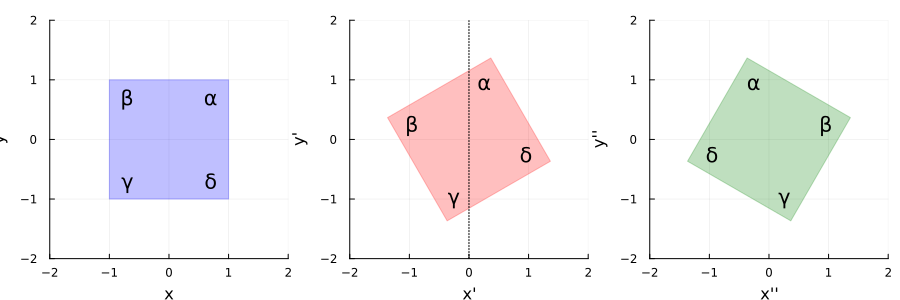
\includegraphics[width=\textwidth]{chained-transformation-1.png}
\end{center}

\vspace{4mm}
{\bf Problem 6 (challenge):} Express the chained transformation from $\bx$ to $\bx''$
as a matrix-vector multiplication. 

\vspace{4mm}
{\bf Strategy:}
You should have the reflection as a matrix-vector product from problem 3,
and you can get the rotation matrix by plugging in $\theta = \pi/6$ to your
answer for problem 1.

\vspace{4mm}
Let the rotation and reflection matrices and the coordinate vector $(x,y)$ be labeled
as follows
\begin{align*}
  R = \begin{bmatrix} r_{11} & r_{12} \\ r_{21} & r_{22} \end{bmatrix}, \quad \quad
  S = \begin{bmatrix} s_{11} & s_{12} \\ s_{21} & s_{22} \end{bmatrix}, \quad \quad
  \bx = \begin{bmatrix} x \\ y \end{bmatrix}.                                                                                                
\end{align*}
Your $R$ and $S$ matrices will have specific numerical values instead of symbols, but I'll
use symbols as above to avoid giving away the answers for previous problems! 
  
\vspace{4mm}
Then the rotation transformation is $\bx' = R \bx$, and the reflection is $\bx'' = S \bx'$,
and the chained transformation is $\bx'' = S \bx' = S(Rx)$. Writing that out in long-hand form,

\begin{align}
  \begin{bmatrix} x'' \\ y'' \end{bmatrix}
                        =
  \begin{bmatrix} s_{11} & s_{12} \\ s_{21} & s_{22} \end{bmatrix}
  \left(\begin{bmatrix} r_{11} & r_{12} \\ r_{21} & r_{22} \end{bmatrix}
  \begin{bmatrix} x \\ y \end{bmatrix} \right) \label{SRx}
\end{align}
Again, you will have specific numebrs for the matrix coefficients instead of symbols.

\vspace{4mm}
Now do across-and-down on the $Rx$ multiplication to get $Rx$ expressed as a vector.
Then do across-and-down on the $S (Rx)$ multiplication. You should end up with a vector
whose components are sums of $x$ and $y$ times some numeric coefficients. Then rewrite
that vector as a single matrix-vector multiplication, where the coefficients go in the matrix,
and the vector is $\bx = \begin{bmatrix} x \\ y \end{bmatrix}$. The answer should look like
\begin{align}
  \begin{bmatrix} x'' \\ y'' \end{bmatrix}
                        =
  \begin{bmatrix} ? & ? \\ ? & ? \end{bmatrix}
  \begin{bmatrix} x \\ y \end{bmatrix} \label{answerform}
\end{align} 
with specific numbers in place of the question marks.
\newpage

\vspace{4mm}
{\bf Problem 7 (challenge):} Do the same as in problem 6, but using symbols rather than
specific numbers for the matrices. Start directly from equation \ref{SRx}, and end up
with something like equation \ref{answerform}. But instead of numbers for the matrix elements,
you will have expressions involving $r_{11},$ $r_{12}$, $\ldots$ and $s_{11},$ $s_{12}$, $\ldots$.


\vspace{180mm}
{\bf A question to ponder:} Why do mirrors reverse images left to right, but not upside down?

\end{document}
